\chapter{Opciones del Men\'u}
   \label{Opciones-del-Menu}

\section{Men\'u ``\textit{Archivo}''}
   \label{Menu-Archivo}

\begin{itemize}
   \item \textbf{Archivo $\rightarrow$ Nuevo}:\index{Nuevo} Elimina todos los
      procedimientos y variables definidos hasta el momento para comenzar un
      nuevo espacio de trabajo. Se abrir\'a una ventana para confirmar la
      eliminaci\'on de todos los procedimeintos y variables:
      \begin{center}
         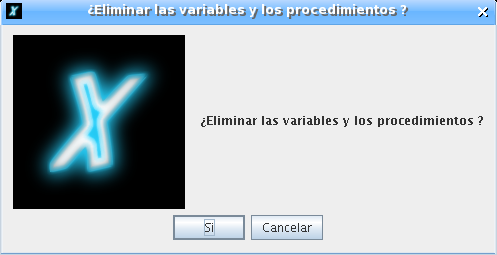
\includegraphics[scale=0.3]{Imagenes/03_Opciones-Menu/MenuNuevo.png}
      \end{center}
   \item \textbf{Archivo $\rightarrow$ Abrir}:\index{Abrir} Carga un archivo
      \textsc{Logo} previamente guardado en disco.
      \begin{center}
         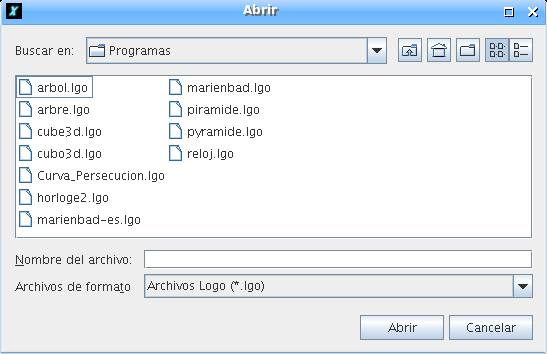
\includegraphics[scale=0.3]{Imagenes/03_Opciones-Menu/MenuAbrir.png}
      \end{center}
   \item \textbf{Archivo $\rightarrow$ Guardar como\ldots{}}:\index{Guardar como ...}
      Graba un archivo (\texttt{.lgo}) de procedimientos definidos hasta ese
      momento en el disco, permitiendo asignarle un nombre. 
      \begin{center}
         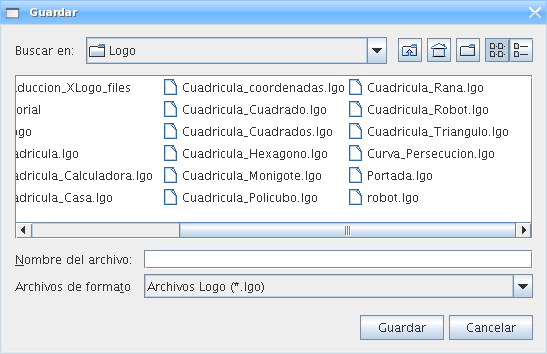
\includegraphics[scale=0.3]{Imagenes/03_Opciones-Menu/MenuGuardar.png}
      \end{center}
   \item \textbf{Archivo $\rightarrow$ Guardar}:\index{Guardar} Graba un archivo
      (\texttt{.lgo}) con los procedimientos definidos hasta ese momento
      en el disco. Esta opci\'on estar\'a deshabilitada mientras no se le haya
      asignado un nombre como se acaba de explicar en el punto anterior.
   \item \textbf{Archivo $\rightarrow$ Capturar imagen $\rightarrow$ Guardar imagen
      como\ldots{}}:\index{Guardar imagen como\ldots} Permite guardar la imagen del
      \'area de dibujo en formato jpg\index{jpg@\texttt{.jpg}} o png.
      \index{png@\texttt{.png}}Para ello, puedes seleccionar previamente una parte
      de la imagen pulsando el bot\'on izquierdo del rat\'on y arrastrando. 
   \item \textbf{Archivo $\rightarrow$ Capturar imagen $\rightarrow$ Imprimir
      imagen}:\index{Imprimir imagen} Permite imprimir la imagen del \'area de
      dibujo. Se puede seleccionar una zona a imprimir tal como se
      explic\'o para \textbf{Guardar}.
   \item \textbf{Archivo $\rightarrow$ Capturar imagen $\rightarrow$ Copiar al
      portapapeles:} \index{Portapapeles} Permite enviar la imagen al portapapeles
      del sistema. Del mismo modo que para \textbf{Imprimir} y \textbf{Guardar},
      se puede seleccionar una zona. Esta opci\'on funciona perfectamente en
      entornos Windows y Mac:
      \begin{center}
         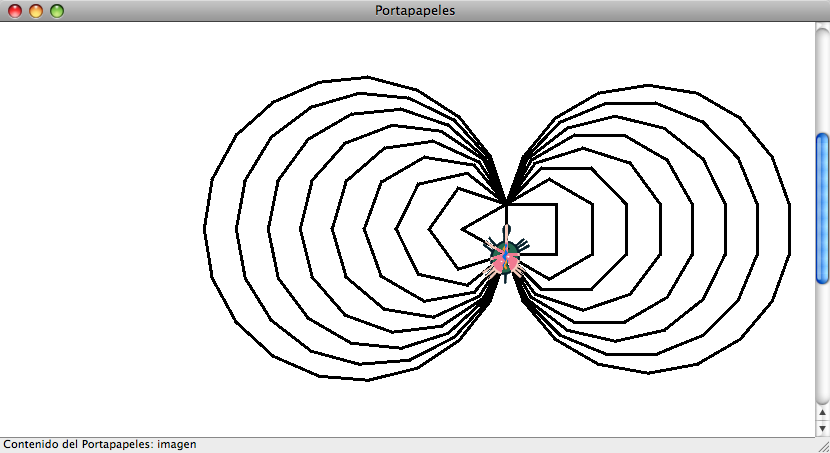
\includegraphics[scale=0.3]{Imagenes/03_Opciones-Menu/Portapapeles_Mac.png}
      \end{center}
      pero no as\'i en entornos Linux (el portapapeles no tiene el mismo
      funcionamiento).
   \item \textbf{Archivo $\rightarrow$ Zona de texto $\rightarrow$ Guardar en
      formato RTF}:\index{Guardar en formato RTF} Guarda el contenido del
      \textbf{Hist\'orico de Comandos} en un fichero con formato RTF \index{RTF}
      (\textit{Rich Text Format}), manteniendo los colores de los mensajes. Si
      no se escribe la extensi\'on \texttt{.rtf}, se a\~nade autom\'aticamente. 
      \begin{center}
         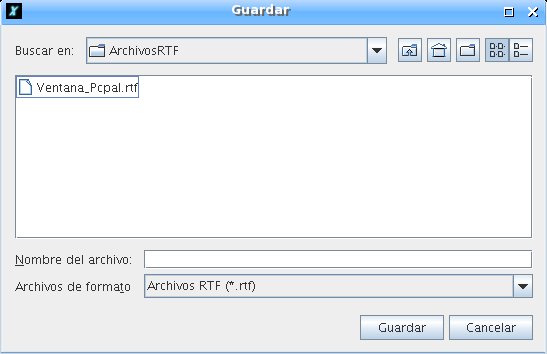
\includegraphics[scale=0.3]{Imagenes/03_Opciones-Menu/Guardar_RTF.png}
      \end{center}
   \item \textbf{Archivo $\rightarrow$ Salir}: \index{Salir} Finaliza la ejecuci\'on
      de \textsc{XLogo}. Tambi\'en puede terminarse la ejecuci\'on desde la L\'inea
      de comandos con la primitiva \texttt{adi\'os}. \index{adi\'os@\texttt{adi\'os}}
\end{itemize}

\section{Men\'u ``\textit{Edici\'on}''}
   \label{Menu-Edicion}
   \index{Edici\'on}

\begin{itemize}
   \item \textbf{Edici\'on $\rightarrow$ Copiar}:\index{Copiar} copia el texto
      seleccionado en el portapapeles. Atajo de teclado: \texttt{Control+C}
   \item \textbf{Edici\'on $\rightarrow$ Cortar}:\index{Cortar} corta el texto
      seleccionado y lo copia en el portapapeles. Atajo de teclado:
      \texttt{Control+X}
   \item \textbf{Edici\'on $\rightarrow$ Pegar}:\index{Pegar} pega el texto desde el
      portapapeles a la l\'inea de comandos. Atajo de teclado:
      \texttt{Control+V}
   \item \textbf{Edici\'on $\rightarrow$ Seleccionar todo}:\index{Seleccionar todo}
      Selecciona todo lo que se encuentra escrito en la
      \textbf{L\'inea de Comandos}.
\end{itemize}

\section{Men\'u ``\textit{Herramientas}''}
   \label{Menu-Herramientas}

\begin{itemize}
   \item \textbf{Herramientas $\rightarrow$ Elegir el color del l\'apiz}:
      \index{Elegir color del l\'apiz} Permite elegir el color con que la
      tortuga dibujar\'a, desde la paleta de colores, mediante una
      definici\'on \texttt{HSB} (\textit{Hue}, \textit{Saturation}, 
      \textit{Brightness} - Tonalidad, Saturaci\'on, Brillo) o desde
      una codificaci\'on \texttt{RVA} (Rojo, Verde y Azul).
      \begin{center}
         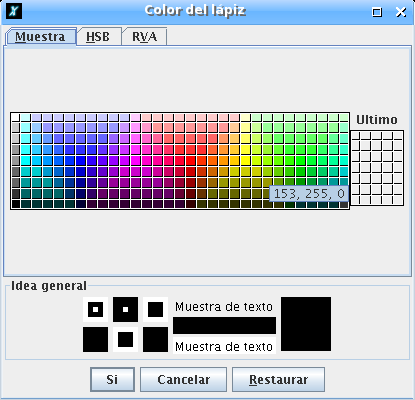
\includegraphics[scale=0.3]{Imagenes/03_Opciones-Menu/ColorLapiz_01.png}
         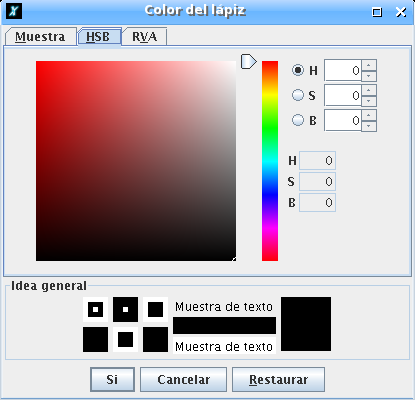
\includegraphics[scale=0.3]{Imagenes/03_Opciones-Menu/ColorLapiz_02.png}
         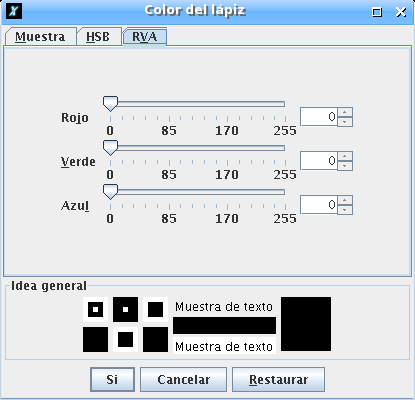
\includegraphics[scale=0.3]{Imagenes/03_Opciones-Menu/ColorLapiz_03.png}
      \end{center}
      Tambi\'en accesible con el comando \texttt{poncolorlapiz}.
      \index{poncolorlapiz@\texttt{poncolorlapiz}} (Secci\'on
      \ref{Propiedades-Tortuga})
   \item \textbf{Herramientas $\rightarrow$ Elegir el color de fondo (papel)}:
      \index{Elegir color del papel} Pone un color como fondo de pantalla,
      con las mismas caracter\'isticas que \textbf{Elegir Color del L\'apiz}.
      Tambi\'en accesible con el comando \texttt{poncolorpapel}.
      \index{poncolorpapel@\texttt{poncolorpapel}} (Secci\'on
      \ref{Propiedades-Tortuga})
   \item \textbf{Herramientas $\rightarrow$ Definir archivos de inicio}:
      \index{Definir archivos de inicio} Permite establecer la ruta a los
      archivos de inicio.
      \begin{center}
         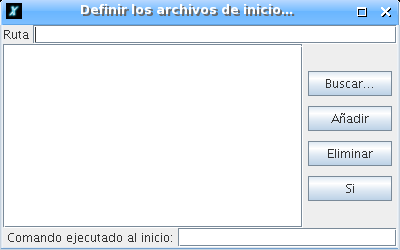
\includegraphics[scale=0.3]{Imagenes/03_Opciones-Menu/DefinirArchivosInicio.png}
      \end{center}
      Cualquier procedimiento contenido en estos archivos
      \texttt{.lgo} \index{lgo@\texttt{.lgo}}
      se convertir\'an en ``\textit{seudo-primitivas}'' del
      lenguaje \textsc{XLogo}. Pero no pueden ser modificadas por el usuario.
      As\'i se pueden definir primitivas personalizadas
      \index{Primitivas personalizadas}.
   \item \textbf{Herramientas $\rightarrow$ Traducir procedimientos}:
      \index{Traducir procedimientos} Abre una caja de di\'alogo que permite
      traducir los comandos \textsc{XLogo} entre dos idiomas. Es muy \'util,
      en particular, cuando se obtienen c\'odigos \textsc{Logo} en ingl\'es
      (de internet, por ejemplo) para expresarlos en el idioma deseado
      (Espa\~nol, Franc\'es, \ldots{})
      \begin{center}
         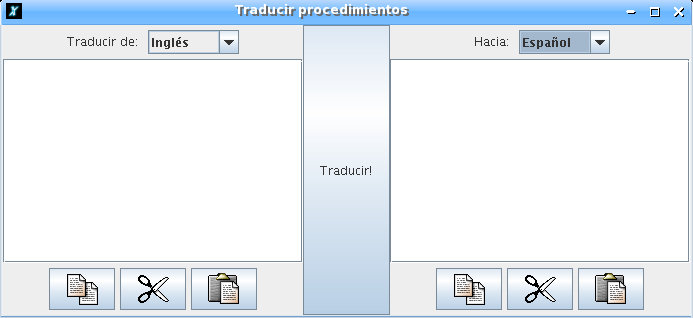
\includegraphics[scale=0.3]{Imagenes/03_Opciones-Menu/TraducirProcedimientos.png}
      \end{center}
   \item \textbf{Herramientas $\rightarrow$ Borra procedimientos}:
      \index{Borrar procedimientos} Abre una caja de di\'alogo que permite
      selccionar el procedimiento que se desea borrar, de una forma m\'as
      sencilla que con la primitiva \texttt{borra}.
      \begin{center}
         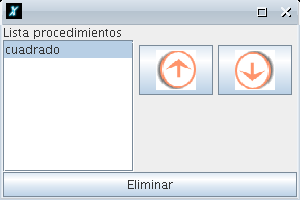
\includegraphics[scale=0.3]{Imagenes/03_Opciones-Menu/BorraProcedimientos.png}
      \end{center}
   \item \textbf{Herramientas $\rightarrow$ Preferencias}:\label{Menu_Preferencias}
      \index{Preferencias}Abre una caja de di\'alogo donde se pueden
      configurar varios aspectos:
      \begin{itemize}
         \item \textbf{General:}
            \begin{itemize}
               \item \textbf{Idioma}: \index{Idioma} Permite elegir entre
                  Franc\'es, Ingl\'es, Espa\~nol, Gal\'es, Portugu\'es,
                  Esperanto, \'Arabe y Gallego. Nota que las primitivas
                  se adec\'uan a cada lenguaje.
               \item \textbf{Aspecto}: \index{Aspecto} Permite definir el
                  aspecto de la ventana \textsc{XLogo}. Est\'an disponibles los
                  estilos ``Windows'', ``Metal'' y ``Motif''.
               \item \textbf{Velocidad de la tortuga}:
                  \index{Velocidad de la tortuga} Si prefieres ver todos
                  los movimientos de la tortuga, puedes reducir la velocidad
                  con la barra deslizante. 
            \end{itemize}
            \begin{center}
               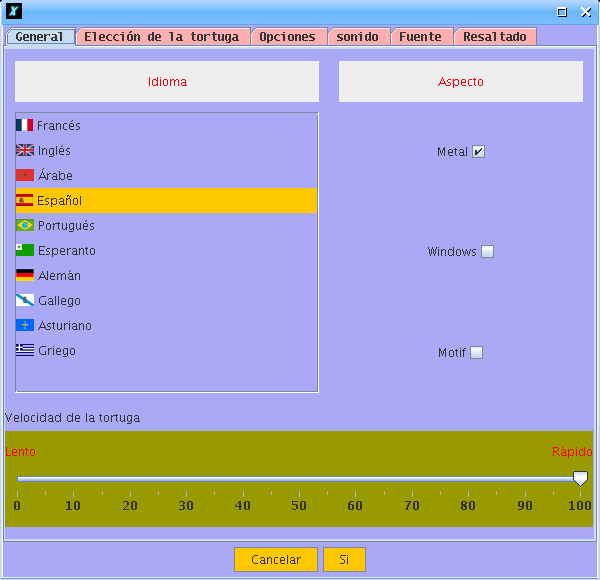
\includegraphics[scale=0.3]{Imagenes/03_Opciones-Menu/Preferencias_01.png}
             \hfill
               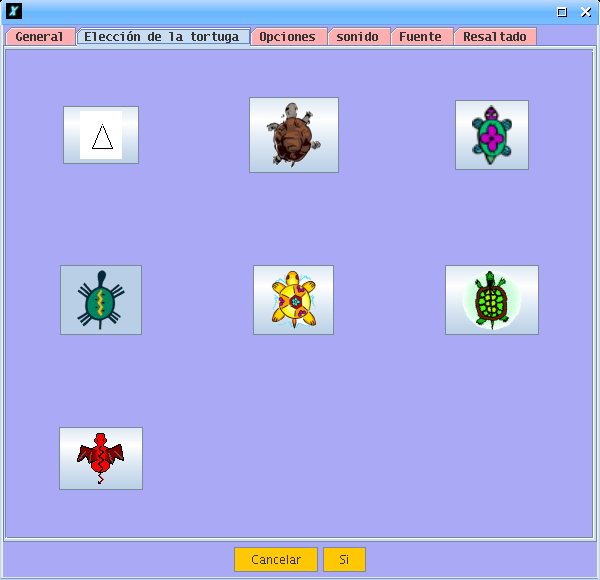
\includegraphics[scale=0.3]{Imagenes/03_Opciones-Menu/Preferencias_02.png}
            \end{center}
         \item \textbf{Elecci\'on de la tortuga}: \index{Figura de la tortuga}
            Elige entre siete tortugas distintas. Tambi\'en accesible con el
            comando \texttt{ponforma} \index{ponforma@\texttt{ponforma}}
            (Secci\'on \ref{Propiedades-Tortuga})
         \item \textbf{Opciones:}
            \begin{center}
               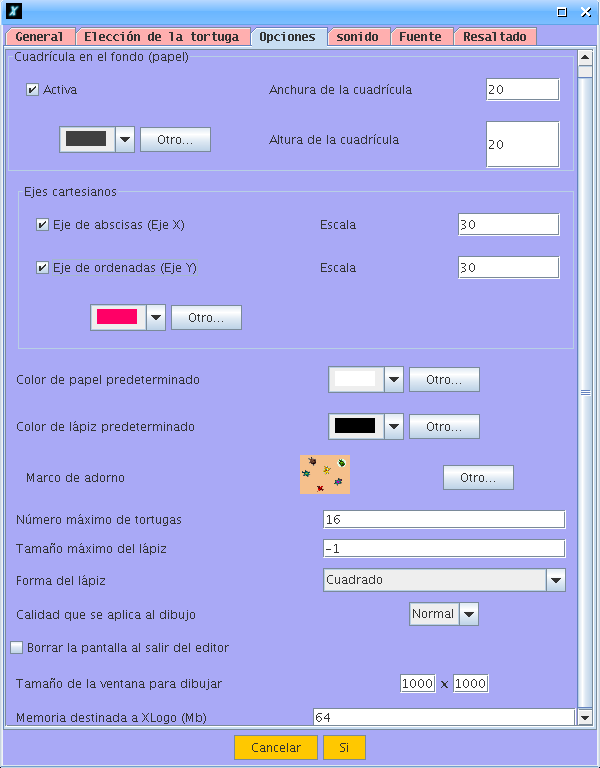
\includegraphics[scale=0.3]{Imagenes/03_Opciones-Menu/Preferencias_03.png}
            \end{center}
            \begin{itemize}
               \item \textbf{Cuadr\'icula en el fondo}:\index{Cuadr\'icula}
                  Establece (o elimina) una cuadr\'icula en el fondo del
                  \'Area de dibujo, as\'i como las medidas y el color de la
                  misma. Tambi\'en accesible con las primitivas 
                  \texttt{cuadricula}\index{cuadricula@\texttt{cuadricula}},
                  \texttt{detienecuadricula} y \texttt{poncolorcuadricula}.
                  \index{detienecuadricula@\texttt{detienecuadricula}}
                  \index{poncolorcuadricula@\texttt{poncolorcuadricula}}
                  (Secci\'on \ref{Propiedades-Tortuga})
               \item \textbf{Ejes cartesianos}:\index{Ejes cartesianos}
                  Muestra (o retira) los ejes cartesianos (X e Y) del \'Area de
                  dibujo, establece su escala (separaci\'on entre marcas) y
                  su color. Tambi\'en accesible con las primitivas
                  \texttt{ejes}\index{ejes@\texttt{ejes}},
                  \texttt{detieneejes}\index{detieneejes@\texttt{detieneejes}},
                  \texttt{ejex}\index{ejex@\texttt{ejex}},
                  \texttt{ejey}\index{ejey@\texttt{ejey}} y
                  \texttt{poncolorejes}\index{poncolorejes@\texttt{poncolorejes}}
                  (Secci\'on \ref{Propiedades-Tortuga}).
               \item \textbf{Color de papel predeterminado}:
                  \index{Color de papel predeterminado} Permite elegir el color
                  por defecto del papel, es decir, el mostrado al iniciar
                  \textsc{XLogo}. 
               \item \textbf{Color de l\'apiz predeterminado}:
                  \index{Color de l\'apiz predeterminado} Permite elegir el color
                  por defecto del l\'apiz, es decir, el utilizado al iniciar
                  \textsc{XLogo}.
               \item \textbf{Marco de adorno}:
                  \index{Marco de adorno} Permite elegir qu\'e marco de adorno
                  se muestra alrededor del \textbf{\'Area de Dibujo}, una
                  imagen o un color s\'olido. Para no superar la memoria
                  asignada, la imagen no puede ocupar m\'as de 100 kb.
                  \begin{center}
                   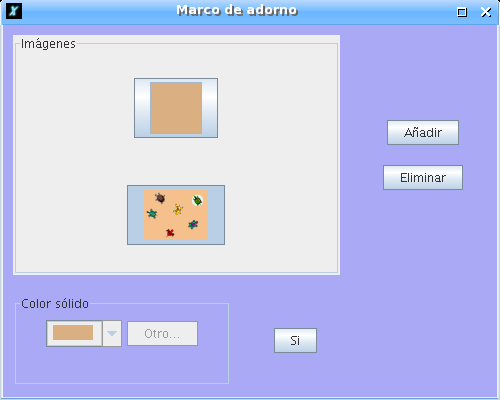
\includegraphics[scale=0.5]{Imagenes/03_Opciones-Menu/Preferencias_Marco.png}
                  \end{center}
               \item \textbf{N\'umero m\'aximo de tortugas}:
                  \index{N\'umero m\'aximo de tortugas} Para el modo
                  multitortuga (secci\'on \ref{Modo-multitortuga}).
                  Por defecto 16.
               \item \textbf{Tama\~no m\'aximo del l\'apiz}:
                  \index{Tama\~no m\'aximo del l\'apiz} Puedes fijar un
                  tama\~no l\'imite para el l\'apiz. Si no se va a utilizar
                  esta limitaci\'on, introduce el n\'umero \texttt{-1} en el
                  recuadro asociado. 
               \item \textbf{Forma del l\'apiz}: \index{Forma del l\'apiz}
                  Cuadrado o Redondo 
               \item \textbf{Tama\~no de la ventana para dibujar}:
                  \index{Tama\~no de la ventana} Puedes establecer un tama\~no
                  personalizado para el \textbf{\'Area de Dibujo}. Por defecto
                  \textsc{XLogo} establece un \'area de 1000 por 1000 pixels.

                  \textbf{Atenci\'on}: seg\'un aumenta el tama\~no de la
                  imagen, puede ser necesario aumentar la memoria destinada
                  a \textsc{XLogo}. Un mensaje de error advertir\'a si ocurre
                  esto.
               \item \textbf{Calidad que se aplica al dibujo}:
                  \index{Calidad del dibujo}Normal, Alto o Bajo. En calidad
                  ``Alta'', no se aprecia ning\'un efecto en
                  particular, pero puede producirse una ralentizaci\'on de la
                  ejecuci\'on.
               \item \textbf{Borrar pantalla al salir del editor}: S\'i o No
               \item \textbf{Tama\~no de la ventana para dibujar}:
                  \index{Tama\~no de la ventana}Determina las dimensiones del
                  \'Area de dibujo.
               \item \textbf{Memoria destinada a \textsc{XLogo}}:
                  \index{Memoria destinada a \textsc{XLogo}} (en Mb) Por
                  defecto, el valor asignado es 64 Mb. Puede ser necesario
                  aumentarlo cuando el tama\~no del \textbf{\'Area de Dibujo}
                  sea demasiado grande. La modificaci\'on de este par\'ametro
                  s\'olo se har\'a efectiva tras cerrar y reiniciar
                  \textsc{XLogo}.

                  \textbf{Atenci\'on}: no aumentar en exceso y/o sin raz\'on
                  este valor, ya que puede ralentizar considerablemente el
                  sistema. Un ejemplo en el que se puede necesitar bastante
                  memoria disponible es al trabajar en el modo 3D com dise\~nos
                  muy complejos.
            \end{itemize}
         \item \textbf{Sonido}: \index{Sonido} La lista de instrumentos que
            puede imitar la tarjeta de sonido a trav\'es de la interfaz
            MIDI. \index{MIDI} Puedes seleccionar un instrumento concreto
            en cualquier momento, mediante la primitiva 
            \texttt{poninstrumento n}.
            \index{poninstrumento@\texttt{poninstrumento}}

            Si usas Windows, esta lista puede estar vac\'ia. Esto se debe
            a que la versi\'on de \textsc{Java} para Windows no incluye los
            \textit{bancos de sonido}, y deben instalarse manualmente. Echa
            un vistazo a la secci\'on \ref{Sonido-Instrumentos-Error}.
            \begin{center}
               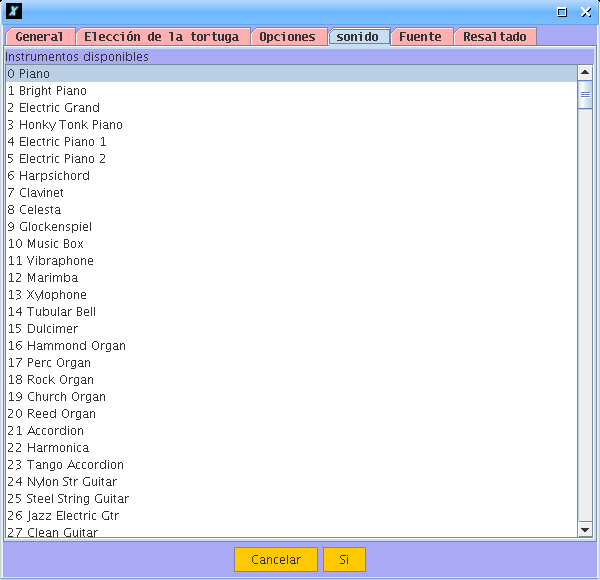
\includegraphics[scale=0.3]{Imagenes/03_Opciones-Menu/Preferencias_04.png}
         \hfill
               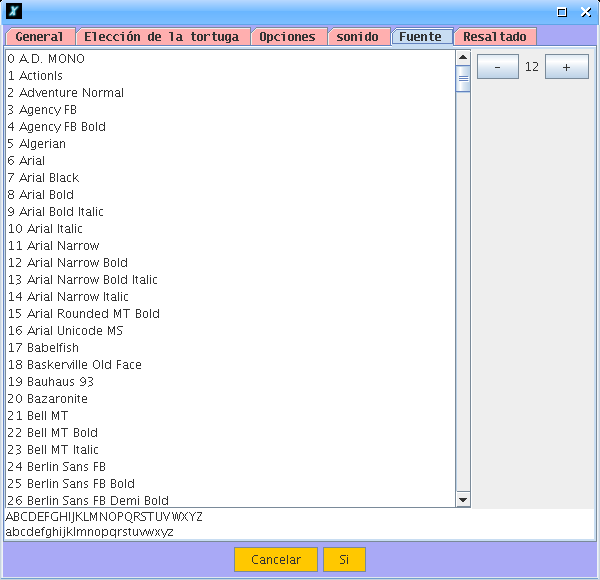
\includegraphics[scale=0.3]{Imagenes/03_Opciones-Menu/Preferencias_05.png}
            \end{center}
         \item \textbf{Fuente}: \index{Fuente} Elige el tipo de letra y su
            tama\~no
            \begin{center}
               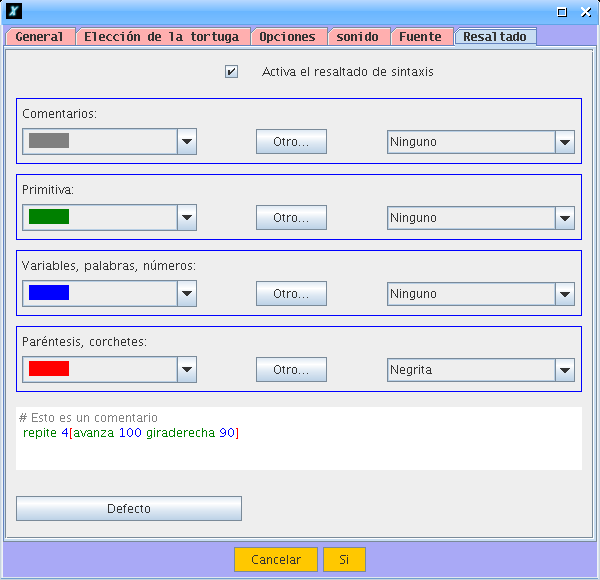
\includegraphics[scale=0.3]{Imagenes/03_Opciones-Menu/Preferencias_06.png}
            \end{center}
         \item \textbf{Resaltado}: \index{Resaltado} Elige los colores que
            se utilizar\'an en el resaltado de primitivas, palabras, variables 
            n\'umeros, par\'entesis y corchetes.
      \end{itemize}
\end{itemize}

\section{Men\'u ``\textit{Ayuda}''}
   \label{Menu-Ayuda}
   \index{Ayuda}

\begin{itemize}
   \item \textbf{Ayuda $\rightarrow$ Licencia}: \index{Licencia GPL}Muestra
      la licencia original GPL (en Ingl\'es) bajo la cual es distribuido este
      programa.
      \begin{center}
         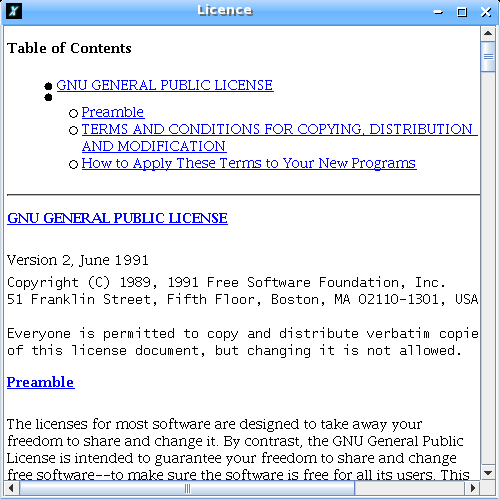
\includegraphics[scale=0.3]{Imagenes/03_Opciones-Menu/Licencia.png}
         \hfill
         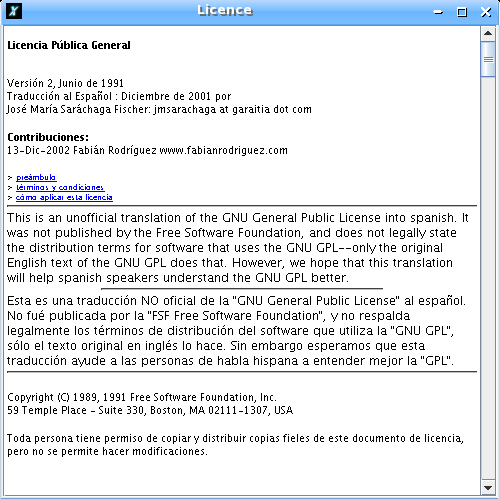
\includegraphics[scale=0.3]{Imagenes/03_Opciones-Menu/Licencia-sp.png}
      \end{center}
   \item \textbf{Ayuda $\rightarrow$ Traducci\'on de la Licencia}:
      \index{Traducci\'on de la Licencia} Refiere a una traducci\'on al
      espa\~nol de la licencia GPL, sin efectos legales, s\'olo como
      referencia para entender la versi\'on en Ingl\'es.
   \item \textbf{Ayuda $\rightarrow$ Traducir XLogo}: \index{Traducir XLogo}
      Abre una ventana para a\~nadir y/o corregir traducciones.
      \begin{center}
         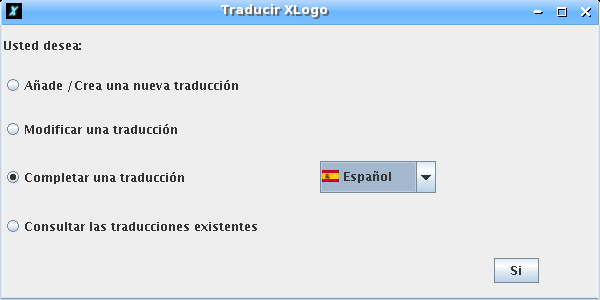
\includegraphics[scale=0.3]{Imagenes/03_Opciones-Menu/Traducir_01.png}
         \hfill
         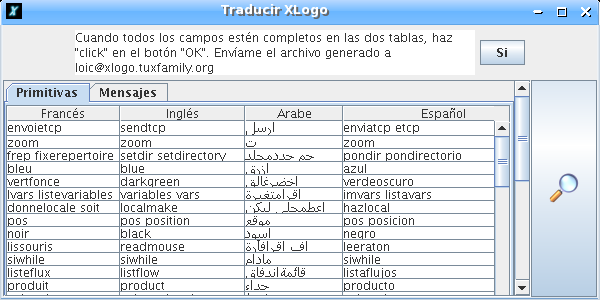
\includegraphics[scale=0.3]{Imagenes/03_Opciones-Menu/Traducir_02.png}
      \end{center}
      Desde ella pueden crearse y/o modificarse tanto las primitivas como
      los mensajes. Una vez creados/modificados, haz \textit{click} 
      \textbf{fuera} de la celda que acabas de escribir y pulsa el bot\'on 
      \texttt{Si}. Se abrir\'a una ventana donde debes elegir el fichero
      de texto donde guardar los cambios y que debes enviar a
      \texttt{loic@xlogo.tuxfamily.org}
      \begin{center}
         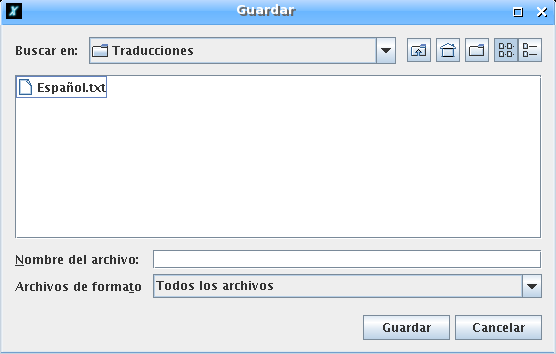
\includegraphics[scale=0.3]{Imagenes/03_Opciones-Menu/Traducir_03.png}
      \end{center}
   \item \textbf{Ayuda $\rightarrow$ Acerca de\ldots{}}: \index{Acerca de ...} Lo de
      siempre \ldots{} y !`!`\texttt{xlogo.tuxfamily.org} para guardar en
      favoritos!! o:)
      \begin{center}
         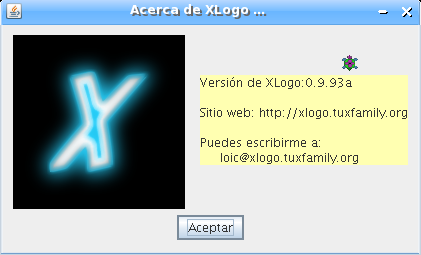
\includegraphics[scale=0.45]{Imagenes/03_Opciones-Menu/Acerca093.png}
      \end{center}
\end{itemize}
